\documentclass{article}%
\usepackage[T1]{fontenc}%
\usepackage[utf8]{inputenc}%
\usepackage{lmodern}%
\usepackage{textcomp}%
\usepackage{lastpage}%
\usepackage[head=40pt,margin=0.5in,bottom=0.6in]{geometry}%
\usepackage{graphicx}%
%
\title{\textbf{Representante de Venezuela en CIDH indicó que la crisis es culpa de EE UU}}%
\author{El Nacional Web}%
\date{04/10/2018}%
%
\begin{document}%
\normalsize%
\maketitle%
\textbf{URL: }%
http://www.el{-}nacional.com/noticias/politica/representante{-}venezuela{-}cidh{-}indico{-}que{-}crisis{-}culpa\_254346\newline%
%
\textbf{Periodico: }%
EN, %
ID: %
254346, %
Seccion: %
Política\newline%
%
\textbf{Palabras Claves: }%
Política, Estados Unidos, OEA, Crisis económica, Gobierno\newline%
%
\textbf{Derecho: }%
18, %
Otros Derechos: %
, %
Sub Derechos: %
\newline%
%
\textbf{EP: }%
NO\newline%
\newline%
%
\textbf{\textit{Larry Lavoe, vocero venezolano en la audiencia, indicó que el país tiene el mejor sistema financiero, sin embargo, no se puede aplicar por los bloqueos y sanciones}}%
\newline%
\newline%
%
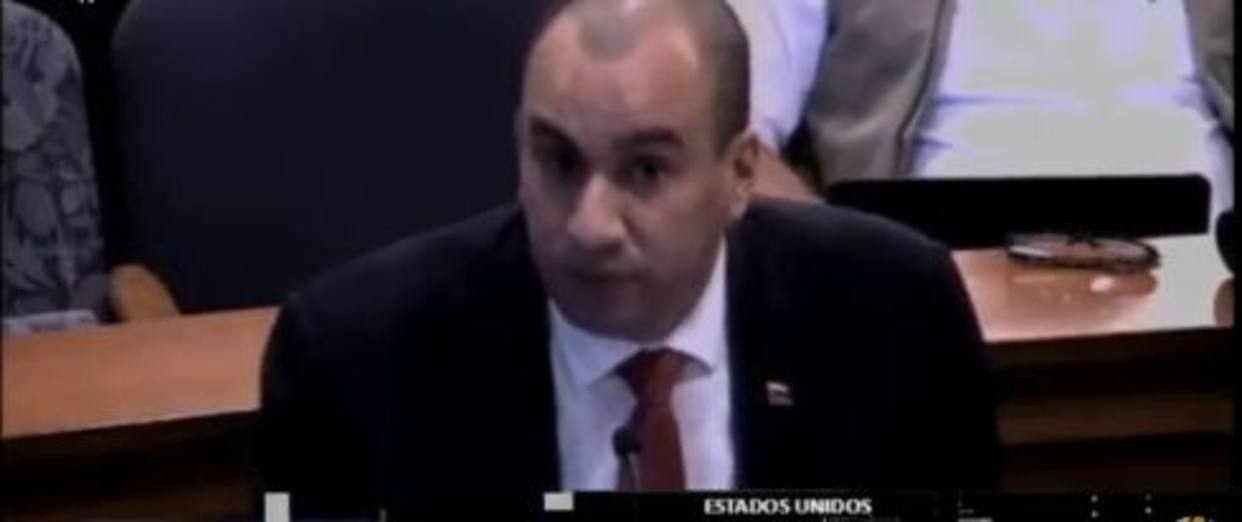
\includegraphics[width=300px]{191.jpg}%
\newline%
%
Larry Davoe, representante de Venezuela en la audiencia de la Comisión Interamericana de los Derechos Humanos (CIDH), aseguró que el país tiene el mejor sistema financiero del mundo. Indicó que no se puede aplicar por las sanciones y los bloqueos de Estados Unidos.%
\newline%
%
“Tenemos que profundizar en las causas que afectan al pueblo. Venezuela ha sido sometida a un mecanismo de agresión económica”, dijo.%
\newline%
%
Laveo explicó que Venezuela tiene la capacidad económica para atender a la población necesitada e informó que se han invertido más de 2.400 millones de dólares en las cajas de alimentos CLAP. A su juicio, la crisis económica y humanitaria del país es consecuencia de las acciones de Estados Unidos.%
\newline%
%
Por otro lado, el representante de Venezuela abordó el tema de los privados de libertad y dijo que los funcionarios del Sistema Bolivariano de Inteligencia Nacional (Sebin) respetan y garantizan los derechos de los recluidos.%
\newline%
%
“El Estado venezolano es el principal interesado en que exista paz”, añadió.%
\newline%
%
\end{document}